\chapter{Présentation de l'entreprise}

Ce chapitre situe Air Liquide Tunisie au sein du groupe Air Liquide, présente ses activités et décrit le service Maintenance dans lequel le stage s'est déroulé. Les informations générales proviennent des sites officiels du groupe ; la description du service repose sur les observations faites sur place.

\section{Le groupe Air Liquide}

Air Liquide est un groupe industriel créé en 1902, à la suite des travaux de Georges Claude sur la liquéfaction de l'air et grâce à la mobilisation de Paul Delorme~\cite{ref1}. Il fournit des gaz, des technologies et des services pour l'industrie et la santé. Selon les données 2025 publiées en mars 2026, le groupe emploie environ 65 000 collaborateurs dans 59 pays~\cite{ref1}.

\section{Air Liquide Tunisie}

\begin{wrapfigure}[13]{r}{0.34\textwidth}
\vspace{-6pt}
\centering
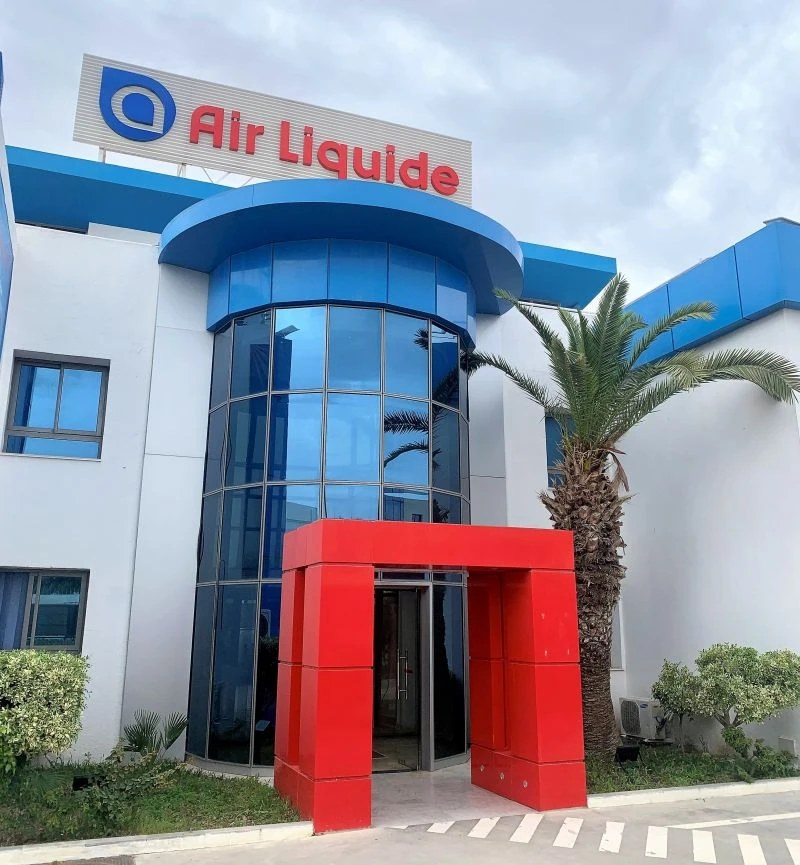
\includegraphics[width=\linewidth]{facade_air_liquide.jpg}
\caption{Façade d'un bâtiment d'Air Liquide Tunisie}
\end{wrapfigure}

Air Liquide est présent en Tunisie depuis 1917~\cite{ref2}. Sa filiale tunisienne compte aujourd'hui 230 collaborateurs, 6 sites de production et 35 points de vente, et sert plus de 16 000 clients, parmi lesquels la plupart des hôpitaux et cliniques du pays ; elle est cotée à la Bourse de Tunis et certifiée ISO 9001, ISO 14001 et FSSC 22000~\cite{ref2}.

Dans le domaine de la santé, Air Liquide Tunisie intervient à l'hôpital (gaz et équipements médicaux), tandis que la santé à domicile est assurée par la filiale VitalAire Tunisie, avec un accompagnement \og{}de l'hôpital au domicile\fg{}~\cite{ref3}. Son offre comprend les gaz médicaux (oxygène médical, air médical reconstitué, dioxyde de carbone), les systèmes de distribution de gaz médicaux et des équipements complémentaires~\cite{ref3}~\cite{ref4}. Le site d'exploitation visité se trouve à la zone industrielle de Charguia II, à Ariana~\cite{ref2}.

\Needspace{7\baselineskip}

{\small\setstretch{1.05}\renewcommand{\arraystretch}{1.3}\arrayrulecolor{ALtexte}
\begin{longtable}{|>{\raggedright\arraybackslash}p{3.29cm}|>{\raggedright\arraybackslash}p{11.32cm}|}
\caption{Activités de santé d'Air Liquide Tunisie (synthèse des sources~\cite{ref2},~\cite{ref3} et~\cite{ref4})}\\
\hline
\rowcolor{ALbleu} \sffamily\bfseries\color{white} Domaine & \sffamily\bfseries\color{white} Contenu (d'après les sites officiels) \\ \hline
\endfirsthead
\caption[]{Activités de santé d'Air Liquide Tunisie (synthèse des sources~\cite{ref2},~\cite{ref3} et~\cite{ref4}) (suite)}\\
\hline
\rowcolor{ALbleu} \sffamily\bfseries\color{white} Domaine & \sffamily\bfseries\color{white} Contenu (d'après les sites officiels) \\ \hline
\endhead
Gaz médicaux & Oxygène médical, air médical reconstitué, dioxyde de carbone, systèmes de distribution de gaz médicaux \\ \hline
\rowcolor{ALgris} Équipements & Équipements cryogéniques et équipements pour installations hospitalières, en complément des gaz \\ \hline
Santé à domicile & Assurée par VitalAire Tunisie, de l'hôpital au domicile \\ \hline
\end{longtable}
}

Les pages officielles consultées ne décrivent pas le service de maintenance des appareils respiratoires : la présentation qui suit repose donc sur les observations réalisées pendant le stage.

\section{Le service d'accueil : le service Maintenance}

Le stage s'est déroulé au service Maintenance (maintenance biomédicale), placé sous la responsabilité de M. Marouane Hassan, responsable génie biomédical. Le service prend en charge les équipements médicaux respiratoires retournés par les patients ou les clients : concentrateurs d'oxygène, appareils de ventilation non invasive (VNI) et appareils de type CPAP. L'équipe de l'atelier comprend notamment deux techniciens, Fares et Maher.

Le plan de réaménagement des ateliers santé du site de Charguia (décembre 2025) et la signalétique des portes montrent l'organisation physique du circuit d'un appareil : une \textbf{salle de retour} (\og{}Retour matériel infecté\fg{}), une \textbf{salle de désinfection}, l'\textbf{atelier de maintenance SAT} et une zone de \textbf{stockage des dispositifs médicaux livrables}. Ce circuit physique est celui que l'application reproduit.

\begin{figure}[!htb]
\centering
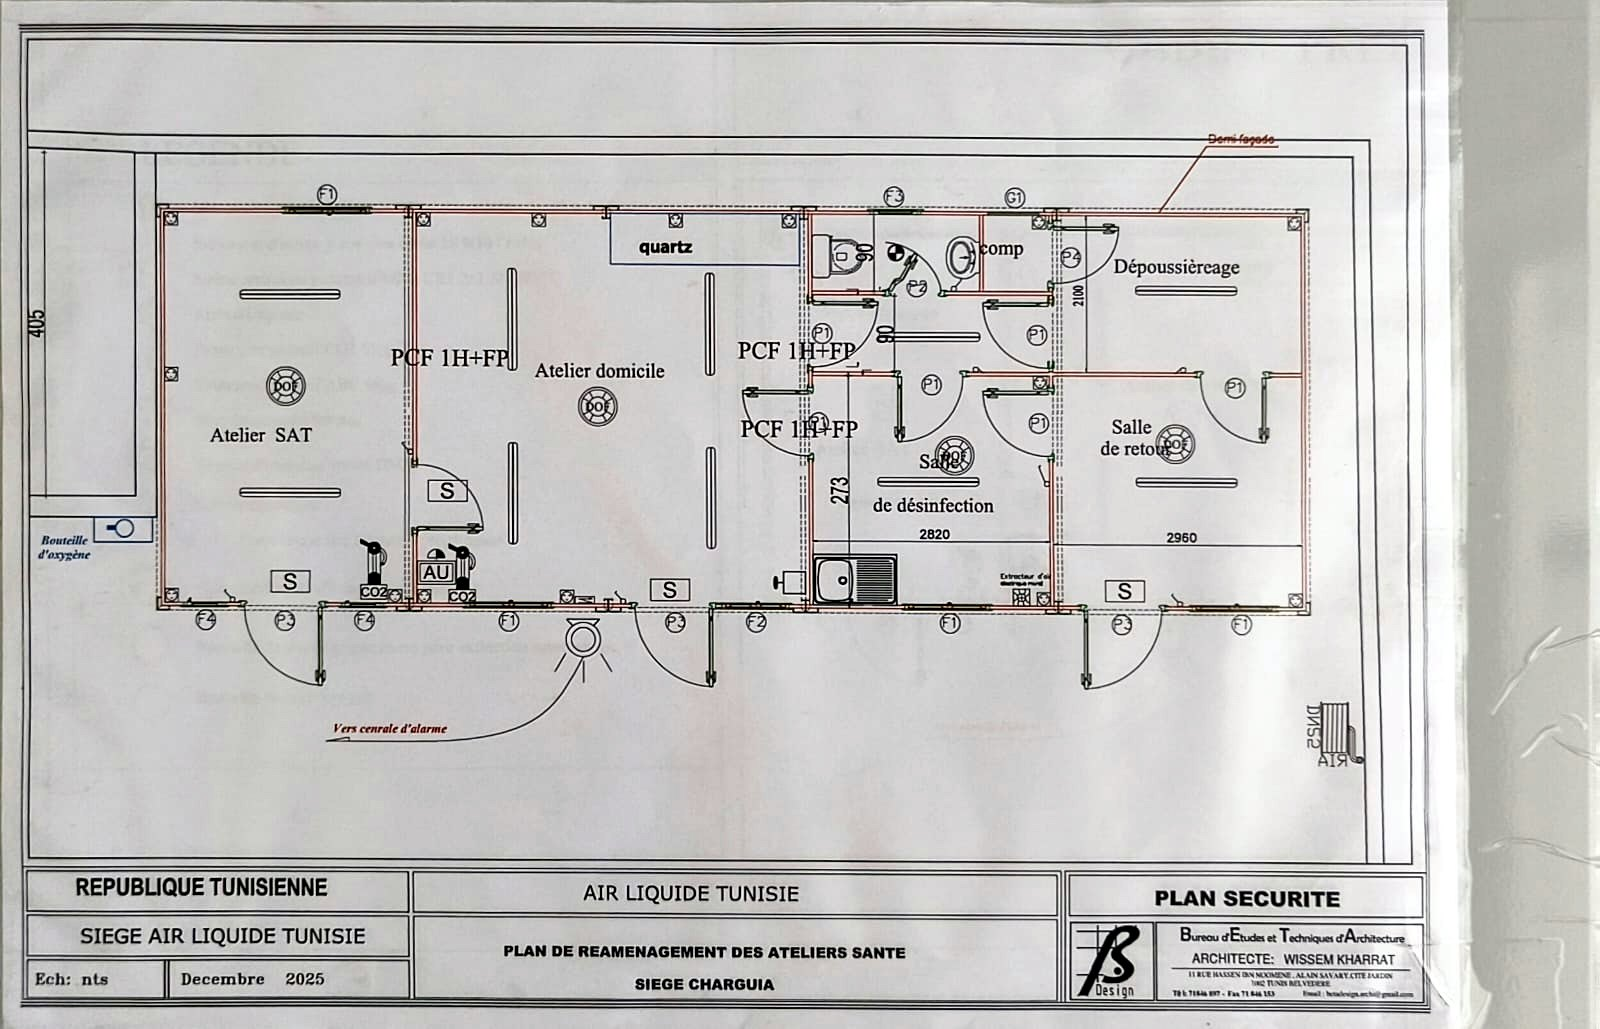
\includegraphics[width=15.5cm,height=11.0cm,keepaspectratio]{plan_ateliers_sante.jpg}
\caption{Plan de réaménagement des ateliers santé, site de Charguia (Air Liquide Tunisie, décembre 2025)}
\end{figure}

\begin{figure}[!htb]
\centering
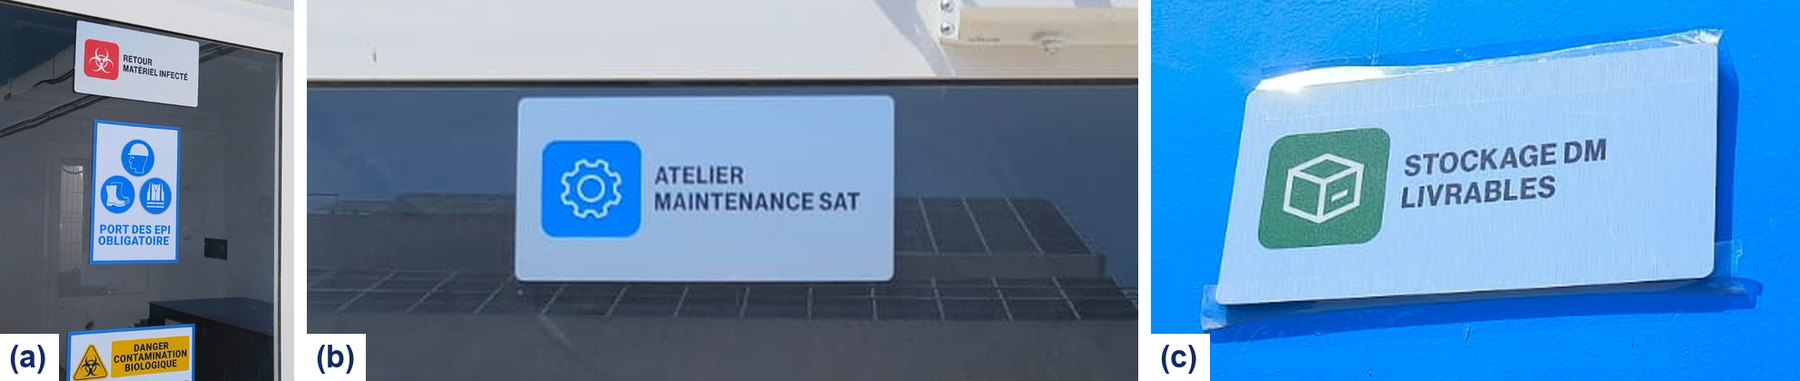
\includegraphics[width=15.5cm,height=6.5cm,keepaspectratio]{signaletique_zones.jpg}
\caption{Signalétique des zones : (a) retour du matériel infecté, (b) atelier de maintenance, (c) stockage des dispositifs médicaux livrables}
\end{figure}

\Needspace{16\baselineskip}
\section{Cadre du stage}

{\small\setstretch{1.05}\renewcommand{\arraystretch}{1.3}\arrayrulecolor{ALtexte}
\begin{longtable}{|>{\raggedright\arraybackslash}p{4.57cm}|>{\raggedright\arraybackslash}p{10.04cm}|}
\caption{Cadre du stage}\\
\hline
\rowcolor{ALbleu} \sffamily\bfseries\color{white} Élément & \sffamily\bfseries\color{white} Information \\ \hline
\endfirsthead
\caption[]{Cadre du stage (suite)}\\
\hline
\rowcolor{ALbleu} \sffamily\bfseries\color{white} Élément & \sffamily\bfseries\color{white} Information \\ \hline
\endhead
Période & du 1\textsuperscript{er} juillet au 1\textsuperscript{er} août 2026 \\ \hline
\rowcolor{ALgris} Entreprise & Air Liquide Tunisie \\ \hline
Service & Maintenance (maintenance biomédicale) \\ \hline
\rowcolor{ALgris} Encadrant professionnel & M. Marouane Hassan, responsable génie biomédical \\ \hline
Équipe d'accueil & Techniciens de l'atelier, dont Fares et Maher \\ \hline
\rowcolor{ALgris} Sujet & Conception et réalisation d'une application de gestion de la maintenance (AirLiquide GMAO+) \\ \hline
\end{longtable}
}

